\section{Diseases}
\DndDropCapLine{Y}{}ou find yourself in a world rife with divine curses, man-made disease and magic anomalies, some of them are listed here, beware to not contract theml for it may spell your end.

\begin{figure}[H]
    \centering
    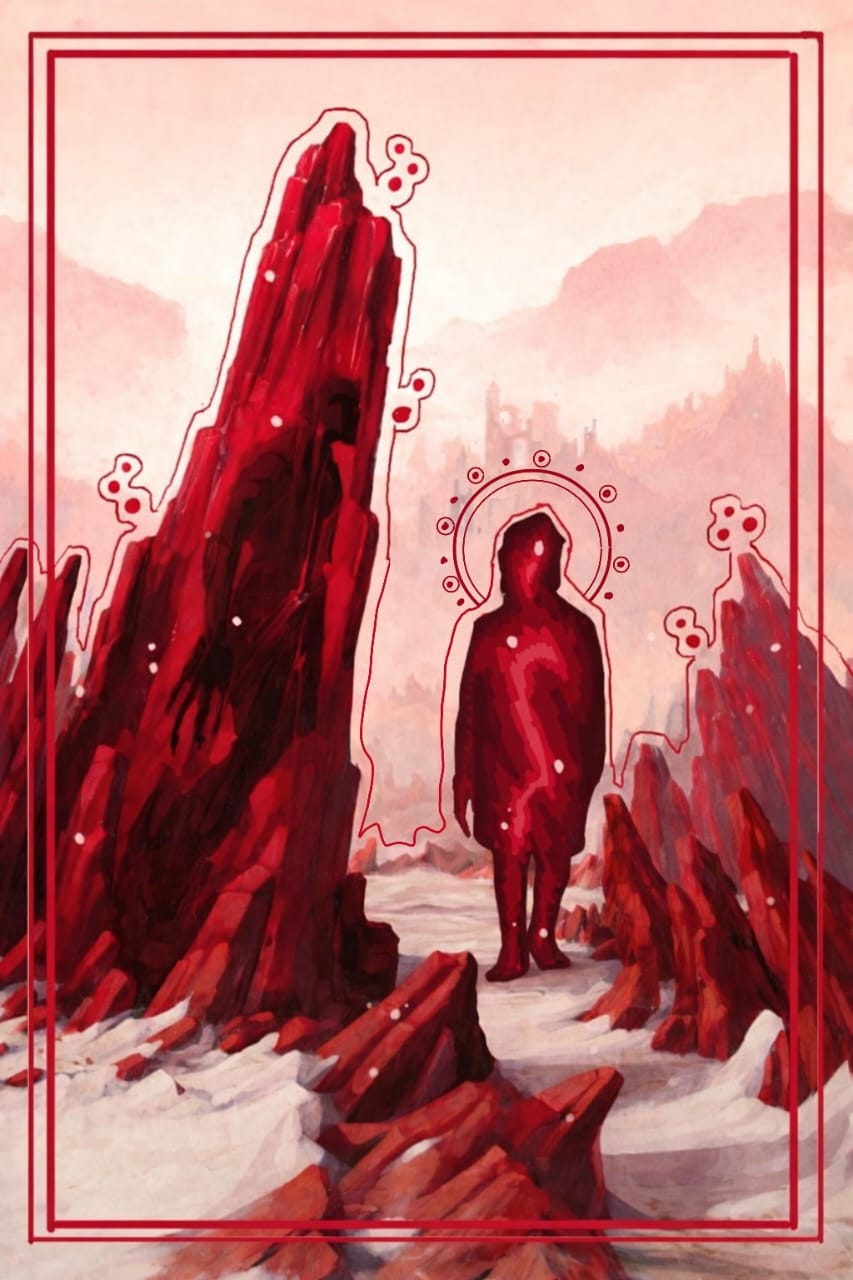
\includegraphics[width=0.6\linewidth]{Images/red_lyr.jpeg}
    \label{fig:placeholder}
\end{figure}

\begingroup
\DndSetThemeColor[PhbMauve]
\begin{DndSidebar}{Pillars of Eternity}
\textit{Streaked with golden pillars and domed roofs, \textbf{Romulon} is a vast and modern city.}
\end{DndSidebar}
\endgroup

\subsection{Lyrium Drawbacks}
\label{main:lyrium}\appendixlink{lyrium}{Appendix IV}{Red Lyrium Enemies}
Blue Lyrium, a magical stimulant used by mages, sorcerers, paladins, eldritch knights etc. is used to empower their spellcasting abilities, in the case of the abyssal tieflings, outright removing the need for any material components, with the exception of warlocks and clerics as their power isn't innate. Red Lyrium, a poor attempt at an artificial substitute to Blue Lyrium, is a chaotic growth of bright ruby crystals found underground in the deep roads. A creation of the Dwerfen Gemmists, abandoned and sealed due to its failed, corrupting behaviour. The Blue Lyrium trade however has provided to be quite lucrative and many mercenary companies and smugglers seek to profit from this dangerous pharmaceutical.

\DndSpellHeader%
  {Rubrilyriasis}
  {Special affliction}
  {Varies (see Exposure)}
  {Self (proximity) or touch}
  {Active Red Lyrium Crystals}
  {Until removed from exposure; progression is permanent}
\textbf{Ambient Exposure (Mind).} If you spend more than \textit{10 minutes near red lyrium}, make a Willpower (Self-Discipline) test (DC 11) or begin hearing \textit{Calling-like voices} urging you to ingest or physically contact red lyrium. Repeat this test each hour you remain near it. Each failure increases the DC of subsequent tests by +2. If you remain away from red lyrium for 3 consecutive hours, the DC resets to 11.

\textbf{Physical Exposure (Body).} If you are physically exposed to red lyrium, make a Constitution (Stamina) test (DC 11). Each failure increases the DC of subsequent tests by +2.

\textbf{Physical Failure Track.} On the 1st failed Constitution test, your skin takes on a reddish hue and you crave more red lyrium. On the 2nd failed test, you grow small red-lyrium nodules and begin to hunch and deform. On the 3rd failed test, you transform into a Red \textbf{Lyrium Horror, Red Lyrium Shadow, or Red Lyrium Behemoth.} On the 4th failed test, you die, overgrown with red lyrium, leaving crystals growing from your fallen form.

\textbf{Cure.} No cure is known; red lyrium contact is treated as an inevitable death sentence. A possible cure could include a \textit{limited or full wish spell}.

\begin{figure}[H]
    \centering
    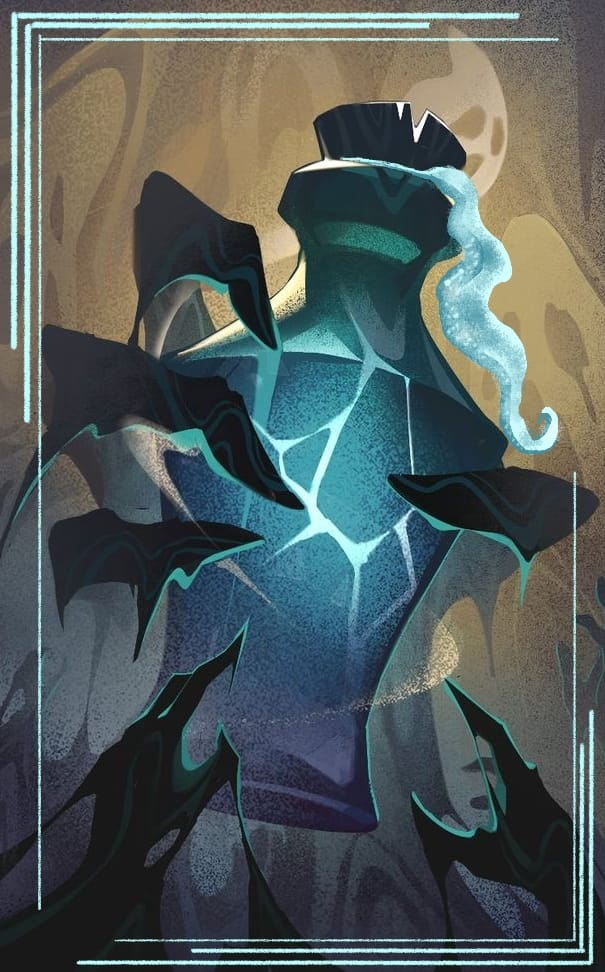
\includegraphics[width=0.6\linewidth]{Images/lyrium.jpeg}
    \label{fig:placeholder}
\end{figure}

\begingroup
\DndSetThemeColor[PhbMauve]
\begin{DndSidebar}{Pillars of Eternity}
\textit{Streaked with golden pillars and domed roofs, \textbf{Romulon} is a vast and modern city.}
\end{DndSidebar}
\endgroup

\DndSpellHeader%
  {Caeruleolyriasis}
  {Special affliction (blue lyrium withdrawal)}
  {1 hour (escalates)}
  {Self}
  {None}
  {Until cured}
When you are separated from a steady supply of \textbf{blue lyrium} (or attempt to stop using it), you suffer \textbf{Caeruleolyriasis} (blue-lyrium withdrawal). While afflicted, you experience fatigue, forgetfulness, a gnawing thirst, and cold hands. As the hunger deepens, paranoia and obsession intensify; you may struggle to separate memory from the present, or waking from dream.

\textbf{Craving Spiral.} At the end of each long rest without blue lyrium, make a Wisdom saving throw (DC 11). On a failure, the DC increases by +2 for subsequent saves until you either consume blue lyrium or complete 3 consecutive long rests without failing. On your \textbf{third failure}, you must use your next available downtime or opportunity to seek blue lyrium, prioritizing it over other goals unless doing so would cause immediate, obvious death.

\textbf{Withdrawal Side-Effect.} Each time you fail the Wisdom saving throw for \textbf{Craving Spiral}, roll a d8 on your withdrawal side-effect table and apply the result until you finish a long rest (or longer, if the table says so).

\textbf{Mental Fog.} While Caeruleolyriasis is active, you have disadvantage on checks made to recall information, track time, or resist intimidation and manipulation that promises relief.

\textbf{Fade Echoes (Full-casters).} If you can cast spells, on a failed save you also hear indistinct voices and suffer brief dizzy spells; on a success, these symptoms lessen after a long rest. Unlike paladins or eldritch knights, mages may recover from the adverse effects with rest and abstinence, at the GM's discretion.

\textbf{Cure.} A healer's regimen, supervised withdrawal, or powerful restorative magic may end Caeruleolyriasis. In settings where lyrium dependence is considered irreversible, treatment only manages symptoms rather than curing them.

\begin{DndTable}[color=PhbLightCyan]{cX}
  \textbf{d6} & \textbf{Withdrawal Side-Effect} \\
  1 & \textbf{Dermal Luminescence.} You shed dim light 5 ft. and have disadvantage on Dexterity (Stealth).\\
  2 & \textbf{Arcano-Dyslexia.} For 1 hour, you must succeed on a DC 12 Intelligence check to read normally. \\
  3 & \textbf{Perceptual Desync.} You have disadvantage on initiative rolls.\\
  4 & \textbf{Fine-Motor Tremor.} You have disadvantage on Dexterity checks made with tools.\\
  5 & \textbf{Scar Irradiation.} You can’t gain temporary hit points.\\
  6 & \textbf{Resistance.} You resist additional withdrawal effects.\\
\end{DndTable}

\begin{figure}[H]
    \centering
    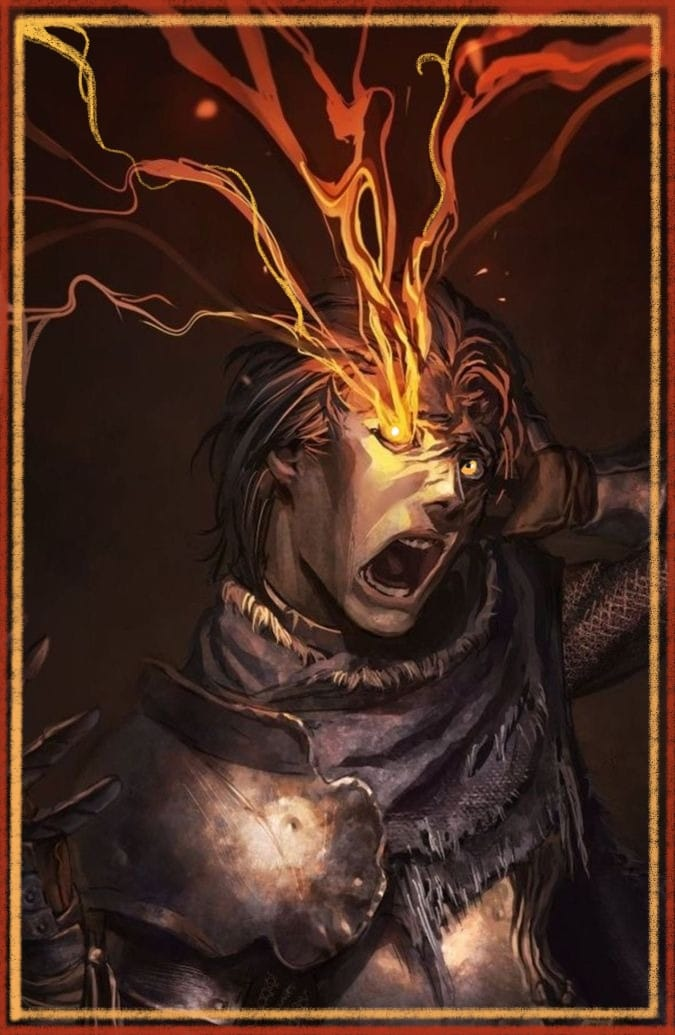
\includegraphics[width=0.6\linewidth]{Images/fr_fl.jpeg}
    \label{fig:placeholder}
\end{figure}

\begingroup
\DndSetThemeColor[PhbMauve]
\begin{DndSidebar}{Pillars of Eternity}
\textit{Streaked with golden pillars and domed roofs, \textbf{Romulon} is a vast and modern city.}
\end{DndSidebar}
\endgroup

\subsection{Purgeflame}
\label{main:purgeflame}\appendixlink{purgeflame}{Appendix I}{Purgeflame Spells}

flavour text

\DndSpellHeader%
  {Empyrosis}
  {Special affliction (the Purgeflame)}
  {Ongoing (slow progression)}
  {Self}
  {None}
  {Until cured (or irreversible)}
Empyrosis is the Purgeflame behind the eyes: a bright, cleansing lie that rewards surrender. It does not spread by time alone. It spreads by \emph{agreement}.

\textbf{Ember Marks.} Empyrosis is tracked with \textbf{Ember Marks} (0--6). You gain Ember Marks primarily by \textbf{giving in} and using Empyrosis gifts. You may also gain 1 Ember Mark at the GM's discretion after major exposure to the Purgeflame.

\textbf{Feeding the Purgeflame.} Each time you use an Empyrosis gift, you gain \textbf{1 Ember Mark} \emph{after the effect resolves}. If the gift caused a creature to trigger Madness Threshold, you gain \textbf{1 additional Ember Mark}.

\textbf{Slow Drift.} At the end of each \textbf{7 days} in which you did \emph{not} use an Empyrosis gift, reduce your Ember Marks by \textbf{1} (minimum 0). This represents the Purgeflame cooling when you refuse it.

\textbf{Point of No Return.} At \textbf{6 Ember Marks}, Empyrosis becomes \textbf{Irreversible}. Your Ember Marks can no longer be reduced by any means, and you cannot be cured. You keep all unlocked gifts, but you are forever considered \emph{touched} by the Purgeflame.

\textbf{Madness Threshold.} When you gain an Ember Mark that brings you to \textbf{3 or more}, you become vulnerable to flare-ups. Whenever you roll initiative, make a Wisdom saving throw (DC 11 + your Ember Marks). On a failure, you become \textbf{Mad}. While Mad, you take \textbf{fire damage equal to twice your CR (or level, minimum 1)} at the start of each of your turns. This damage cannot be reduced or ignored in any way. When you become Mad, you are \textbf{stunned} until the end of your next turn, then the Madness ends.

\textbf{Staged Gifts (Once per Long Rest).} As your Ember Marks rise, Empyrosis unlocks gifts. Each gift can be used \textbf{once per long rest}. Using any gift feeds the Purgeflame as described above.

\textbf{Stage I (Ember scars 1+):} \emph{Purgeflare Cone}

\textbf{Stage II (Ember scars 2+):} \emph{Cry of Shabriel}

\textbf{Stage III (Ember scars 3+):} \emph{Unendurable Purge}

\textbf{Stage IV (Ember scars 4+):} \emph{Inescapable Purge}

\textbf{Stage V (Ember scars 5+):} \emph{Purging Inferno}

\textbf{Cure (Unique).} Empyrosis can be cured only by bathing in the waters of the \textbf{Lazerian Oasis}. A full immersion for at least 10 minutes during a long rest removes all Ember Marks and ends Empyrosis \emph{if and only if} you have not reached the Point of No Return.

\begin{figure}[H]
    \centering
    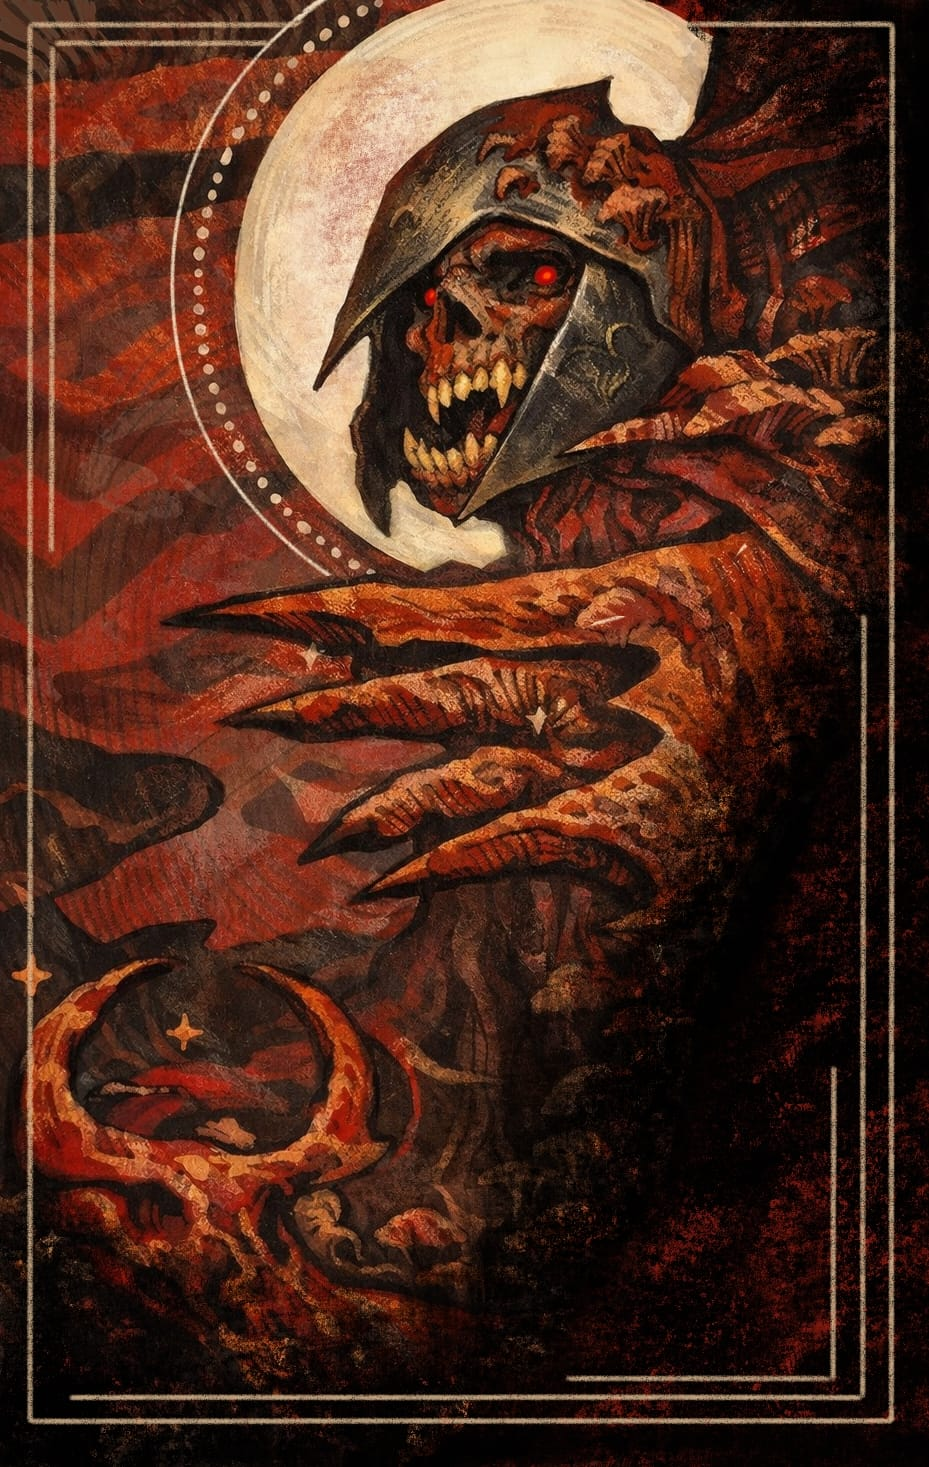
\includegraphics[width=0.6\linewidth]{Images/rot.jpeg}
    \label{fig:placeholder}
\end{figure}

\begingroup
\DndSetThemeColor[PhbMauve]
\begin{DndSidebar}{Pillars of Eternity}
\textit{Streaked with golden pillars and domed roofs, \textbf{Romulon} is a vast and modern city.}
\end{DndSidebar}
\endgroup

\medskip

\subsection{Red Rot}
\label{main:redrot}\appendixlink{redrot}{Appendix II}{Red Rot Spells}

It acts as an incurable, infectious disease that decays the bodies and minds of living things. The manifestation of the outer deity of rot, this 

\DndSpellHeader%
  {Apoptosia}
  {Special affliction (Red Rot)}
  {Ongoing (slow progression)}
  {Self}
  {Rot-infested Material}
  {Until cured (or irreversible)}
Apoptosia is a strain of the \textbf{Red Rot}: a plague-rot that consumes flesh, spoils vitality, and flowers in damp, blighted places. It spreads slowly, but it tightens fastest when you \emph{use} it.

\textbf{Rotwound.} Track Apoptosia with \textbf{Rotwound} (0--5).

\textbf{Contracting the Blight.} When you suffer major exposure to the Red Rot (wading in rot, breathing spores, being struck by a rot attack), make a Constitution saving throw (DC 12). On a failure, gain \textbf{1 Rotwound}.

\textbf{Feeding the Blight.} Each time you use a \textbf{Plagueboon}, you gain \textbf{1 Rotwound} after the effect resolves. This is the core rule: \emph{power strengthens the grip}.

\textbf{Rotting Pulse.} Whenever you gain a Rotwound, you take \textbf{2d6 necrotic damage}. While you have \textbf{3+ Rotwound}, you take \textbf{1d4 necrotic damage} at the start of each of your turns.

\textbf{Odd-Stage Boons.} At Rotwound \textbf{1, 3, and 5}, you gain a boon.

\textbf{Point of No Return.} At \textbf{Rotwound 4}, Apoptosia becomes \textbf{Irreversible}. Your Rotwound can no longer be reduced, and you cannot be cured by any means.

\textbf{Cure and Mitigation (Before 4).} Before Rotwound 4, Apoptosia can be cured or reduced by powerful cleansing rites and remedies at the GM's discretion.

\medskip

\textbf{Stage I (Rotwound 1).} \textbf{Boon: Spore-Sense.} You gain advantage on Perception checks to detect diseased, blighted, or poisonous creatures and terrain.
You unlock the Plagueboon \emph{Touch of Decay} (Once per Long Rest).

\textbf{Stage II (Rotwound 2).} Fever-dreams gnaw your rest. You have disadvantage on checks to resist exhaustion caused by sleeplessness or forced marches.

\textbf{Stage III (Rotwound 3).} \textbf{Boon: Blight Exultation.} Once on each of your turns, when you deal necrotic or acid damage, add \textbf{+1d4} to one damage roll.
You unlock the Plagueboon \emph{Carrion-Breath} (Once per Long Rest).

\textbf{Stage IV (Rotwound 4).} \textbf{Irreversible.} Your body begins to warp with subtle ways as the blight becomes you. You have disadvantage on Wisdom saving throws against fear and charm, but advantage on constitution saves against being poisoned.

\textbf{Stage V (Rotwound 5).} \textbf{Boon: Crown of Bloom.} You gain resistance to \textit{necrotic damage}.
You unlock the Plagueboon \emph{Abyssal Bloom} (Once per Long Rest).

\subsection{Lycanthropy}
\label{main:lycanthropy}\appendixlink{lycanthropy}{Appendix III}{Carlislean Lycanthrope (Monster Class)}

Carlisle was a wretched, fainthearted man of no renown, who wearied of being kicked aside and went begging for strength. In the old wood he found the Dread Wolf, and took its bargain: stout sinew and a predator’s bite, in return for a heart that would sooner turn coat than stand fast. The curse didn’t end with Carlisle, it clung to teeth and bloodlines, spreading wherever desperate people wanted strength more than they wanted to stay themselves.

\DndSpellHeader%
  {Canis Hysteria}
  {Special curse-disease (Carlislean strain)}
  {Ongoing (stage progression)}
  {Self}
  {Physical Wound caused by a werewolf}
  {Until cured, transformed, or sealed}

\textbf{Origin.} The first werewolf was \textbf{Carlisle}, a human cursed by the \textbf{Dread Wolf}, a neutral evil outer god of \textbf{treachery, tyranny, and ambition}. All Carlislean werewolves descend from this single curse-line.

\textbf{Stages.} Track the curse from \textbf{Stage 1} to \textbf{Stage 5}. Stages 1--3 progress like a disease. Stages 4--5 are metamorphosis.

\textbf{Stage Advancement (1--3).} After each \textbf{long rest} while infected, make a Constitution saving throw (DC 12). On a failure, advance by 1 stage (maximum Stage 3 by disease alone).

\textbf{Human Hearts (3 $\rightarrow$ 5).} Eating a \emph{fresh humanoid heart} cannot advance you from Stage 1 to Stage 3. It \textbf{only} advances you from \textbf{Stage 3 to Stage 5} (one stage per heart, maximum one heart per long rest).

\textbf{Coronation of the Wolf (Stage 5 Seal).} To become a \textbf{full werewolf}, you must \textbf{kill another werewolf and feast on its heart}. If you are Stage 3 or higher, doing so immediately advances you to \textbf{Stage 5} and you become \textbf{sealed}.

\textbf{Full Moon Trial.} On each \textbf{full moon}, you transform at dusk and must succeed on a Wisdom saving throw (DC 14 + your current stage) or be compelled to hunt a heart to \emph{quicken or solidify} the curse. 

\textbf{Temporary Transformation (Stages 1--3).} During the full moon you may transform into a hybrid form. While transformed, you have:
\begin{itemize}
\item \textbf{Multiattack} (2 attacks).
\item \textbf{Resistance} to bludgeoning, piercing, and slashing damage from \textbf{nonmagical, nonsilver} sources.
\item \textbf{Bite (Healing).} Once per turn, when you hit with your bite, you regain hit points equal to the damage dealt.
\end{itemize}

\textbf{Stage 1: Keen Flesh (Human Form).}
\begin{itemize}
\item \textbf{Predator Senses.} Advantage on Perception checks relying on smell, hearing, or sight.
\end{itemize}

\textbf{Stage 2: Raw Hunger (Human Form).}
\begin{itemize}
\item \textbf{Craving.} If you begin a long rest without having eaten \textbf{fresh raw meat} that day, you start the rest with \textbf{1 level of exhaustion} (removed if you eat raw meat before the rest ends).
\end{itemize}

\textbf{Stage 3: Waxing Madness (Human Form).}
\begin{itemize}
\item \textbf{Moon-Pull.} During the \textbf{three nights leading up to the full moon}, you have disadvantage on Wisdom and Charisma saving throws.
\item \textbf{Threshold.} Disease progression stops here; only hearts (or the Coronation) push you further.
\end{itemize}

\textbf{Stage 4: Permanent Hybrid (Point of No Return).}
From this stage onward you are always partly changed: heavier musculature, more hair, sharper teeth, and a predator's stare. This is the \textbf{point of no return}; the curse cannot be cured by ordinary means.
\begin{itemize}
\item \textbf{Hardened Frame.} Strength +1.
\item \textbf{Magical Darkvision.} Darkvision 60 ft (or +30 ft if you already have it).
\end{itemize}

\textbf{Stage 5: Class Overwrite.} When you reach Stage 5, you gain levels equal to your current level of the \textbf{Carlislean Lycanthrope} monster class as though you were a \textbf{Gestalt character}. If you were\textit{ already a Gestalt character}, you\textit{ appropriately replace one of your current classes}.
\begin{figure}[H]
\centering
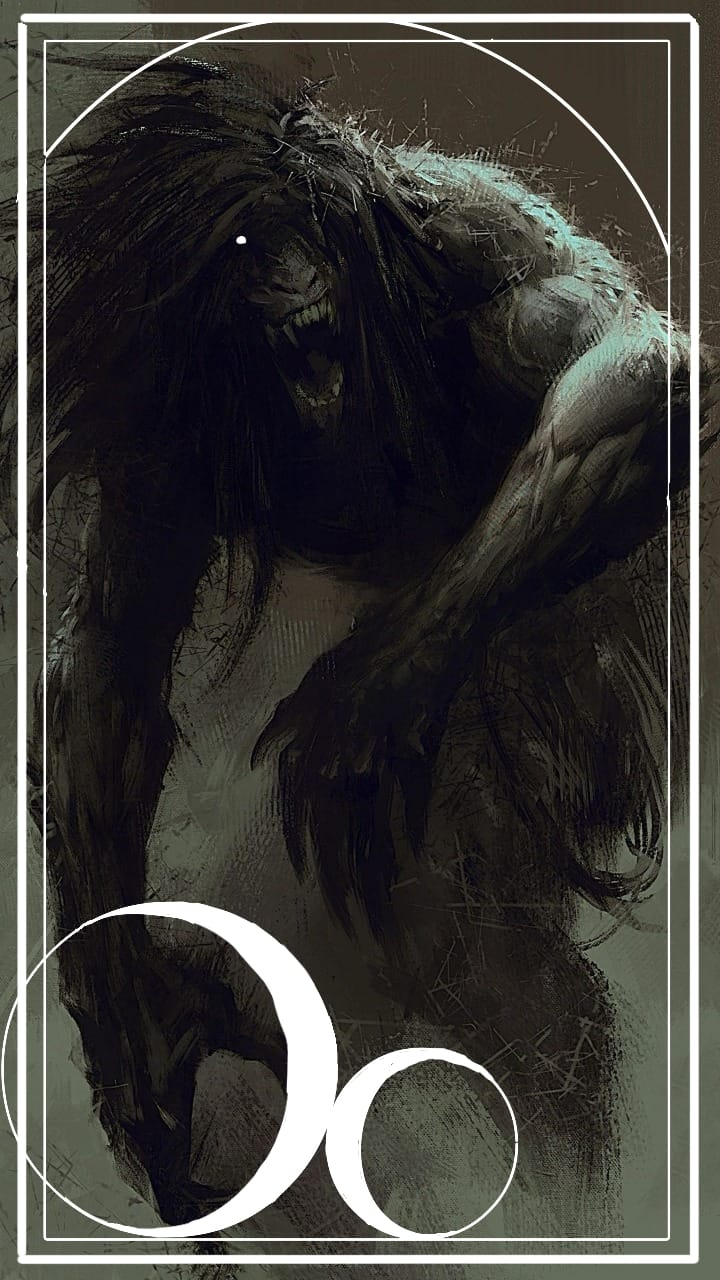
\includegraphics[width=0.2\textwidth]{Images/Werwulf.jpeg}
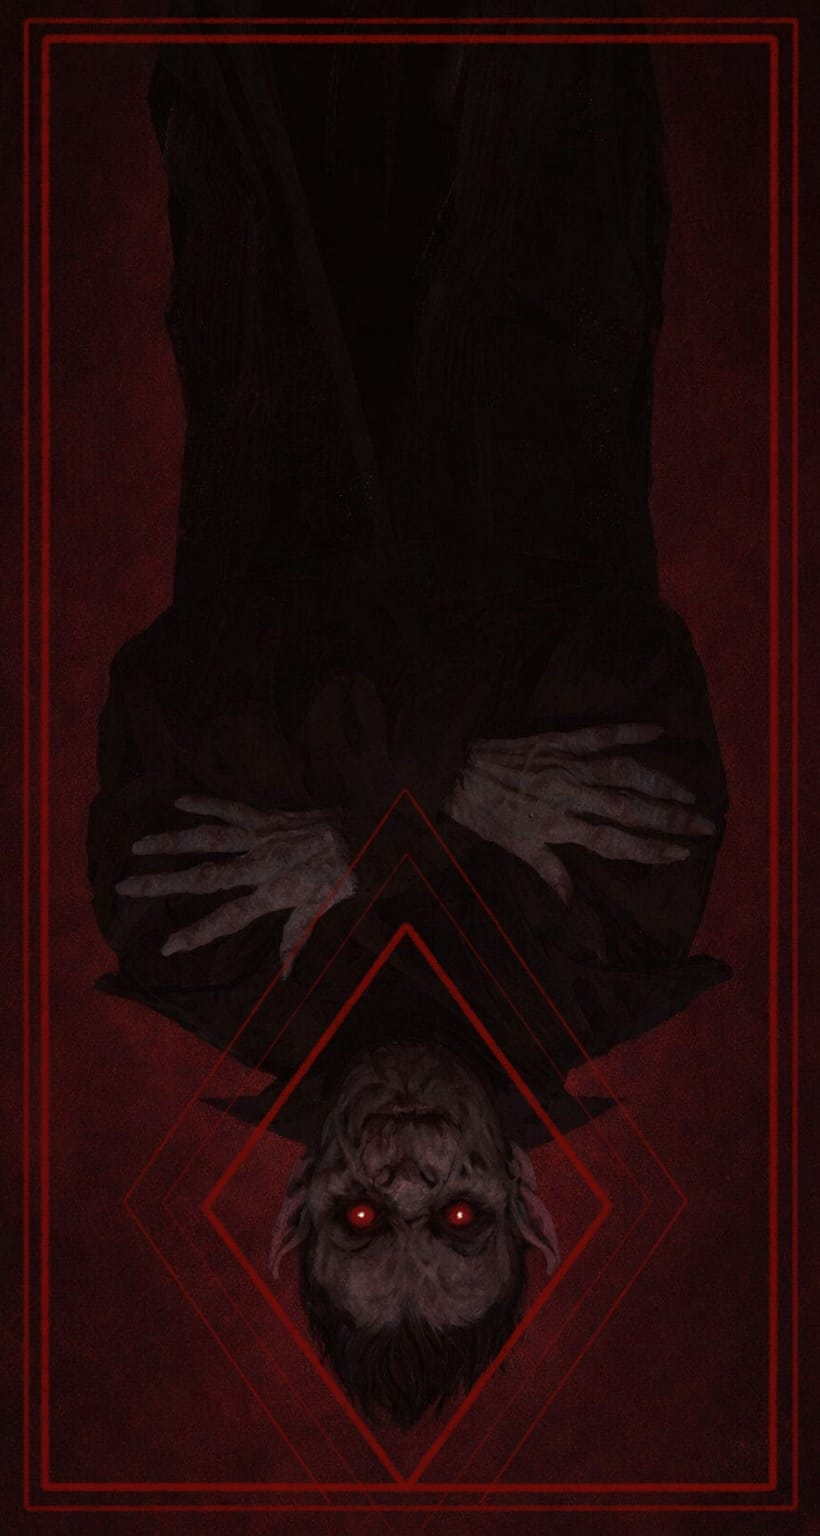
\includegraphics[width=0.19\textwidth]{Images/VAMP.jpeg}
\end{figure}

\begingroup
\DndSetThemeColor[PhbMauve]
\begin{DndSidebar}{Pillars of Eternity}
\textit{Streaked with golden pillars and domed roofs, \textbf{Romulon} is a vast and modern city.}
\end{DndSidebar}
\endgroup

\subsection{Dhampirism}

Dhampirs stand between life and death, endlessly tested by vicious hunger. Most inherit the condition through a vampiric bloodline, but it can also arise when a mortal \textbf{drinks a vampire's blood} and survives the taste.

\DndSpellHeader%
  {Sanguinare Dhampiris}
  {Special affliction}
  {Slow (stage-based)}
  {Self}
  {M (vampire blood, consumed)}
  {Until completed}

\textbf{Strain (Blood-Determined).} Your strain is determined by the \textbf{vampire blood} you consumed. You do not choose it.
\begin{itemize}
\item \textbf{Crystalline.} Iridescent and brittle-skinned; (\emph{Brittle Bones} manifests at Stage 3.)
\item \textbf{Chiropterine.} Bat-like and hairy; heightened awareness and keen reflexes. (\emph{Sunlight Sensitivity} manifests at Stage 3.)
\end{itemize}

\subsubsection{Progression:}
This is a light transformation. After meaningful exposure (GM discretion), such as consuming vampire blood, surviving a vampire's bite, or repeated feeding, make a Constitution saving throw (DC 12). On a failure, advance 1 stage (maximum Stage 3). On a success, you do not advance and take 3d6 necrotic damage as your body rejects the cursed blood.

\medskip

\textbf{Stage 1: Blood-Echo.}
Your body remembers the taste of death, and your senses sharpen.
\begin{itemize}
\item \textbf{Heightened Senses.} You gain advantage on Wisdom (Perception) checks.
\end{itemize}

\textbf{Stage 2: Half-Death.}
The change becomes visible: pallor, sharpened features, and a predatory stillness.
\begin{itemize}
\item \textbf{Darkvision.} You gain darkvision out to 60 feet.
\item \textbf{Life-Draining Bite.} You gain a bite attack that deals \textbf{2d4} damage and heals you for the damage dealt. This bite's damage becomes \textbf{2d6} at character level 4, \textbf{2d8} at level 8, and \textbf{2d10} at level 12.
\item \textbf{Strain Trait (emerges).}
\begin{itemize}
\item \textbf{Crystalline: Tough.} You gain the benefits of the feat: \textbf{tough} and \textbf{resistance to non-magical bludgeoning, piercing and slashing damage.}
\item \textbf{Chiropterine: Dread Ambusher.} You gain a \textbf{dread ambusher} feature from \textbf{Gloomstalker Rangers}.
\end{itemize}
\end{itemize}

\textbf{Stage 3: True Dhampir (Strain Weakness Manifests).}
You are now fully dhampir; hunger is no longer a symptom but the rest of your undead life.
\begin{itemize}
\item \textbf{Strain Weakness.}
\begin{itemize}
\item \textbf{Crystalline: Brittle Bones.} You become vulnerable to thunder damage.
\item \textbf{Chiropterine: Sunlight Sensitivity.} While in sunlight, you have disadvantage on attack rolls and on Wisdom (Perception) checks that rely on sight and gain vulnerability to radiant damage.
\end{itemize}
\end{itemize}

\subsection{Vampirism}

Vampires are cursed creatures of the night, spawn of the two original vampires. A vampire's bite can seed a living body with a cursed strain. The strain does not advance by chance or fortitude, but by \textbf{indulgence}: the curse grows stronger each time you feed it what it truly wants.

\DndSpellHeader%
  {Sanguinare Vampiris}
  {Special affliction}
  {Slow (stage-based)}
  {Self}
  {M (an infecting vampire bite)}
  {Until completed}

\textbf{Strain (Bite-Determined).} Your strain is determined by the \textbf{vampire} that turned you. You do not choose it.
\begin{itemize}
\item \textbf{Crystalline.} Iridescent and brittle-skinned; the curse sets like glass beneath your skin.
\item \textbf{Chiropterine.} Bat-like and hairy; the curse sharpens you into something nocturnal.
\end{itemize}

\subsubsection{Feeding and Progression:}
\begin{itemize}
\item \textbf{Human or Elf Blood.} Each time you knowingly drink \textbf{human or elf blood}, you advance \textbf{1 stage} (maximum Stage 5).
\item \textbf{Animal Blood.} Drinking \textbf{animal blood} does \textbf{not} advance the affliction.
\item \textbf{Stage 3 Gate.} While at \textbf{Stage 3}, you \textbf{cannot} advance to Stage 4 by feeding on mortals. The \textbf{only} way to reach Stage 4 is to drink the blood of your \textbf{primogenitor} (the vampire that turned you), either by \textbf{their consent} or by \textbf{taking it by force}.
\item \textbf{Stage 4 to 5.} Once you are at \textbf{Stage 4}, advancing to \textbf{Stage 5} requires \textbf{human or elf blood} as normal (animal blood still does not advance you).
\end{itemize}

\textbf{Vampire Spawn.} At Stages \textbf{1--3}, you are considered a \textbf{vampire spawn} for the purposes of this affliction's fiction and consequences (GM discretion).

\textbf{Urge Checks (Vampire Spawn Only).} At Stages \textbf{1--3}, when you have a clear opportunity to drink \textbf{human or elf blood} (GM discretion), you must succeed on a Wisdom saving throw or give in.
\begin{itemize}
\item \textbf{DC.} The DC is \textbf{12 + your current stage}.
\item \textbf{On a failure.} You drink if you can, and if you do, the affliction advances as normal.
\item \textbf{On a success.} You resist for now; you do not drink unless you choose to.
\end{itemize}

\medskip

\textbf{Stage 1: Blood-Echo.}
Your body remembers the taste of death, and your senses sharpen.
\begin{itemize}
\item \textbf{Heightened Senses.} You gain advantage on Wisdom (Perception) checks.
\end{itemize}

\textbf{Stage 2: Half-Death.}
The change becomes visible: pallor, sharpened features, and a predatory stillness.
\begin{itemize}
\item \textbf{Darkvision.} You gain darkvision out to 60 feet. If you already have darkvision, increase its range by 30 feet.
\item \textbf{Life-Draining Bite.} You gain a bite attack that deals \textbf{2d4} damage and heals you for the damage dealt. This bite's damage becomes \textbf{2d6} at character level 4, \textbf{2d8} at level 8, and \textbf{2d10} at level 12.
\item \textbf{Strain Trait (emerges).}
\begin{itemize}
\item \textbf{Crystalline: Tough.} You gain the benefits of the feat: \textbf{tough} and \textbf{resistance to non-magical bludgeoning, piercing and slashing damage.}
\item \textbf{Chiropterine: Dread Ambusher.} You gain a \textbf{dread ambusher} feature from \textbf{Gloomstalker Rangers}.
\end{itemize}
\end{itemize}

\textbf{Stage 3: True Vampire (Point of No Return).}
You are now truly vampire; hunger is no longer a symptom, but the rest of your undead life.
\begin{itemize}
\item \textbf{Strain Weakness (manifests).}
\begin{itemize}
\item \textbf{Crystalline: Brittle Bones.} You become vulnerable to thunder damage.
\item \textbf{Chiropterine: Sunlight Sensitivity.} While in sunlight, you have disadvantage on attack rolls and on Wisdom (Perception) checks that rely on sight and gain vulnerability to radiant damage.
\end{itemize}
\end{itemize}

\textbf{Stage 4: Half-Death (Deepening).}
The half-life tightens its grip: your body runs colder, your cravings louder, your instincts faster.
\begin{itemize}
\item \textbf{Life-Draining Bite (improves).} When you hit with your bite, you may choose to deal \textbf{necrotic damage} instead of its normal type; the healing still applies.
\item \textbf{Strain Trait (deepens).}
\begin{itemize}
\item \textbf{Crystalline: Tough (hardened).} If damage dealt to you is \textbf{less than your character level + your proficiency bonus}, you take no damage.
\item \textbf{Chiropterine: Dread Ambusher (honed).} You gain \textbf{flying speed equal to half of your walking speed.} and may use your \textbf{bite attack as a bonus action once per combat.}
\end{itemize}
\end{itemize}

\textbf{Stage 5: True Vampire (Ascendant).}
The curse finishes its work. You are a perfected predator, held together by hunger and old blood.
\begin{itemize}
\item \textbf{Heightened Senses (perfected).} You also gain advantage on Wisdom (Survival) checks made to track creatures by scent.
\item \textbf{Strain Weakness (unchanged, absolute).}
\begin{itemize}
\item \textbf{Crystalline: Brittle Bones.} You remain vulnerable to thunder damage.
\item \textbf{Chiropterine: Sunlight Sensitivity.} While in sunlight, you have disadvantage on attack rolls and on Wisdom (Perception) checks that rely on sight and gain vulnerability to radiant damage.
\end{itemize}
\end{itemize}

\subsection{Usurper's Flesh}

A profane divine disease that clings to the flesh like a slow, sacred ruin. Known commonly as \textbf{Usurper's Flesh}, it deadens skin, whitens scar tissue, erodes the body's natural limits, and leaves the afflicted looking less diseased than wrongly remade.

\DndSpellHeader%
  {Corpus}
  {Special affliction (divine flesh-disease)}
  {Ongoing (slow progression)}
  {Self}
  {Forbidden Knowledge toward the divine}
  {Until cured (or irreversible)}
Corpus, more commonly called \textbf{Usurper's Flesh}, is a malignant divine disease brought on by contact with \textbf{forbidden knowledge of apotheosis}: truths, rites, and revelations concerned with mortal ascension into godhood. It is said that divinity rejects mortal flesh, and that those who reach too far are remade from the extremities inward. The disease advances slowly and often painlessly at first, which makes it all the more dangerous; by the time it is plain to see, it has usually rooted itself deeply.

\textbf{Corpus Limb.} Track Corpus with \textbf{Corpus Limb} (0--5). Each stage marks the disease taking hold in another part of the body: \textbf{left hand, right hand, torso, legs, then head}.

\textbf{Contracting the Disease.} When you \textbf{learn, decipher, witness, or internalize forbidden knowledge} associated with mortal divinity, apotheotic rites, stolen godhood, or similar blasphemous revelations, make a Constitution saving throw (DC 12). On a failure, gain \textbf{1 Corpus Limb}.

\textbf{Aggravating the Disease.} Each time you study such knowledge further, perform a rite of ascension, or willingly expose yourself to relics, texts, visions, or teachings tied to mortal godhood while infected, make a Constitution saving throw (DC 12). On a failure, gain \textbf{1 Corpus Limb}.

\textbf{Flesh Numbness.} Whenever you gain a Corpus Limb, you take \textbf{1d4 necrotic damage}. As more of the body is claimed, sensation dulls, scar tissue thickens, and movement becomes increasingly stiff and unnatural.

\textbf{Odd-Stage Adaptations.} At Corpus Limb \textbf{1, 3, and 5}, you gain a minor adaptation.

\textbf{Point of No Return.} At \textbf{Corpus Limb 3}, once the disease reaches the \textbf{torso}, Corpus becomes \textbf{Irreversible}. Your Corpus Limb can no longer be reduced, and you cannot be cured by ordinary magical means.

\textbf{Amputation and Cure (Before 3).} Before Corpus Limb 3, Corpus may be cured by \textbf{cutting off the affected limb} before the disease spreads further. Rare restorative rites, careful long-term treatment, or specialized alchemy may also reduce or cure the disease at the GM's discretion.

\medskip

\textbf{Stage I (Corpus Limb 1, Left Hand).} \textbf{Adaptation: Deadened Flesh.} You gain advantage on saving throws against disease.
The \textbf{left hand} loses feeling, pales, and begins to stiffen. You have disadvantage on Dexterity checks made with that hand alone, at the GM's discretion.

\textbf{Stage II (Corpus Limb 2, Right Hand).} The \textbf{right hand} begins to show the same numbness and waxen lesions. You have disadvantage on Dexterity checks requiring fine hand movements, and minor injuries to the hands may go unnoticed until they worsen.

\textbf{Stage III (Corpus Limb 3, Torso).} \textbf{Adaptation: Hardened Tissue.} You gain advantage on saving throws against being poisoned.
The disease spreads across the \textbf{torso}, thickening scar tissue over the ribs, back, and abdomen. Your breathing grows shallow and your flesh becomes unnaturally firm in places. \textbf{Corpus is now irreversible.}

\textbf{Stage IV (Corpus Limb 4, Legs).} The \textbf{legs} stiffen as numbness and lesions settle deep into the joints and muscle. Your speed is reduced by \textbf{10 feet}, and you have disadvantage on Charisma (Persuasion) checks as the disease becomes impossible to conceal.

\textbf{Stage V (Corpus Limb 5, Head).} \textbf{Adaptation: Usurping Body.} The first time you would gain a level of exhaustion each Long Rest, you may ignore it.
The disease reaches the \textbf{head}: pale patches creep up the neck and scalp, the face grows visibly altered, and sensation dulls in the lips, ears, or eyelids. Your flesh is now unmistakably overtaken: numb, scarred, pale, and shaped more by the disease than by nature.
